\lecture{LECTURE: IP Addressing}{08-11-22}{09:00}{Amanda}{Zoom}

\section*{Introduction to Internet Protocol}
The Internet Protocol (IP) is a connectionless protocol with best effort delivery. It has no built in data recovery capabilities. IP uses the IP addressing system which is a hierarchical, logical system which is highly scalable. The IP address is the address that sends data to specific computers in the form of packets and it can either be used in the form of static IP addresses or dynamic IP addresses (which get allocated by the Dynamic Host Configuration Protocol, DHCP).

\subsection*{Review of Functions of Internet Protocol}
IP has rules of communication; creates packets; aids the movement of packets across the network; performs one st of tasks when transmitting data and another set of tasks when receiving data.

\section*{IP Addresses}
IP addresses are always known outside of the domain which the device is within, this is different to MAC addresses which are generally only known within the domain which the device is on. IP is more commonly used to identify where the packet is going. MAC addresses are burnt into the Network Interface Card of a device whereas a IP address is assigned to a device and can change. 

Similar to postal addressing, there are two areas of IP addressing. The network ID is similar to a street name and the host ID is similar to a house number. 
\subsection*{Fields of IP Addresses}
IP addresses have three key fields. 
\subsubsection*{Unique x bit address}
In IPv4, this is 32 bit and in IPv6, this is 128 bit. This address is unique to each node on the network. Originally IPv4 had enough possible permutations for every device which was internet connected. Now there are too many devices so IPv6 was introduced. This gives many more potential addresses, in theory enough for every internet connected device.
\subsubsection*{Subnet Mask}
This is a 32-bit pattern used to identify the network and host addresses. Each device does not have a unique subnet mask.
\subsubsection*{Default Gateway}
This is optional. It identifies the address of the router used to access another network outside of your own network, over the internet.

\section*{IP Data Transmission}
\subsection*{Sending Data}
This section assumes IP has already broken the data to be transmitted down into a packet.

The first step of sending data is to establish if the destination is on the same network or a remote network. This is achieved using Addressing Resolution Protocol (ARP), which will use a broadcast to determine if the address is on the same domain at layer three of the reference model. ARP will then translate the IP address of the recipient into its MAC address to aid communication at the data link layer.

If the destination is local, the node can initiate direct communication. Otherwise, the communication must be via a gateway (router). Once the packet is prepared, it is passed to the Network Access Layer which transmits the packet to the connection media where the packet can begin its journey to the destination.

\subsection*{Receiving Data}
When the packet arrives at the Network Access Layer of the receiving node, the datagram is checked for corruption and the that the address is correct. If all is okay, then the Network Access Layer extracts the data and passes it to the designated protocol. 

The IP address gets checked for corruption, this is done by comparing the IP addresses and it ensures that the packet has been delivered to the correct destination.

The instruction set is then checked to determine the next action. This could be to deliver the data to the next layer (TCP or UDP).

\section*{IP Header}
Each packet contains a header as well as the actual data. The header is constructed on the sending computer and it contains information that is used by the protocols and layers. A header has several distinct units of information known as fields.

The IP Header contains, the IP address of the sending computer; the IP address of the destination computer and a set of instructions. As the packet travels through the switches/ routers, the header is examined and updated. 
\subsection*{Detailed Contents of the Header}
\begin{figure}[H]
    \centering
    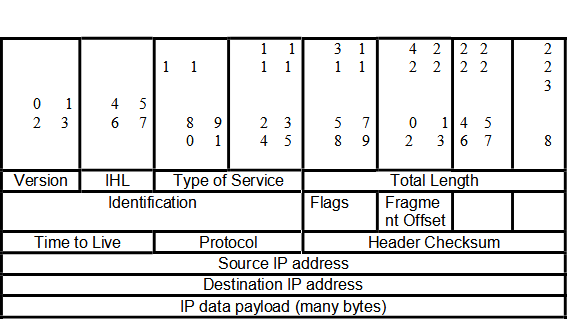
\includegraphics[width=0.8\textwidth]{assets/packet-header.png}
\end{figure}
Headers are at least 20 bytes.
\subsubsection*{Versions}
This identifies the IP version used by this packet (e.g. IPv4 or IPv6).
\subsubsection*{Internet Header Length}
IHL shows the length of the IP header in 32 bit words.
\subsubsection*{Type Of Service}
This gives special routing information requirements. For example
\begin{itemize}
    \item Low or Normal delay
    \item Normal or High throughput
    \item Normal or High readability
\end{itemize}
\subsubsection*{Total Length}
This identifies the length of the packet in octets. The length includes the IP header and the data.
\subsubsection*{Identification}
This gives each packet a unique identifier, in the form of an incrementing sequenced number.
\subsubsection*{Flags}
This indicates fragmentation possibilities of the packet. DF indicates Don't Fragment and MF indicates More Fragments, 0 indicates no more fragments or there was no fragments.
\subsubsection*{Fragment Offset}
This is a numeric value assigned to each fragment, which is used to reassemble the fragments.
\subsubsection*{Time To Live (TTL)}
This is the time in seconds or router hops that the datagram can survive. Routers decrement this field by one as the packet passes through them or by the number of seconds that the datagram is delayed. When the field reaches nought, the datagram is discarded.
\subsubsection*{Protocol}
This holds the protocol address where the IP should deliver the data.
\subsubsection*{Header Checksum}
This holds a 16-bit calculated value to verify the validity of the header.
\subsubsection*{Source IP address}
This is the address of the sending device which is used by the destination IP to verify delivery.
\subsubsection*{IP Data Payload}
This is the data to be delivered. Its size is variable.

\section*{IDs}
Every computer has a unique IP address. This is guided by the public and private addressing rules.

Every computer on a LAN has the same \textit{network ID}. Within that network, each computer will have a unique \textit{host ID}. When these two are combined, they create the IP address.

\subsection*{Servers}
Servers can have multiple IP addresses, this is due to the fact that they can have multiple NICs. Each individual network adapter is a point of contact and therefore known as a node. Therefore each Host ID corresponds to each individual node. 

\section*{IP Address Structure}
\textit{This section only looks at IPv4}

An IP address uses 32 bits, this is hard to remember. The IP address is then broken down into 4 groupings known as octets. Each octet contains 8 binary bits converted into a decimal (this will be a number between 0 and 255).

\section*{IP Address Classes}
A 32 bit binary number has 4 billion different permutations, this means there are 4 billion different IPv4 addresses.

A 128 bit binary number has 340282366920938463463374607431768211456 different permutations, this means there are 340 duodecillion IPv6 addresses.

TCP/IP does not support quite that number. The addresses have been broken down into smaller groups known as classes. These refer to different types of network IDs.

IP addresses are assigned based on the needs of the organisation. They are based on a classes A - C public IP addresses. There are two other classes, D and E however these have different uses.

\subsection*{Class A}
This contains 8 network ID bits and 24 host ID bits. Class A can support 16,777,216 computers.

The leftmost bit is always 0, The leftmost 8 bits comprise the network ID. The rightmost 24 bits contain the host ID.
\begin{verbatim}
NNNNNNNN.HHHHHHHH.HHHHHHHH.HHHHHHHH
255.0.0.0
\end{verbatim}
A subnet is used to differentiate the network ID form the host ID. This is assigned to networks that support large numbers of hosts.

\subsection*{Class B}
This contains 16 network ID bits and 16 host ID bits. It supports 65,536 computers.

The leftmost bit is always 1 and the next bit is always 0.

It is assigned to medium sized networks and a subnet mask is used to differentiate the network ID and host ID.

\begin{verbatim}
NNNNNNNN.NNNNNNNN.HHHHHHHH.HHHHHHHH
255.255.0.0
\end{verbatim}

\subsection*{Class C}
This contains 24 network ID bits and 8 host ID bits. It supports 256 computers.

The leftmost two bits are 1 and the third bit is 0.

It is assigned to small networks and a subnet mask is used to differentiate between the network ID and host ID.
\begin{verbatim}
NNNNNNNN.NNNNNNNN.NNNNNNNN.HHHHHHHH
255.255.255.0
\end{verbatim}

\subsection*{Class D}
The four left most bits start with 1110. This is used for multicasting.

\subsection*{Class E}
This is an experimental class.

The five leftmost bits start with the pattern 11110.